% http://tex.stackexchange.com/questions/11866/compile-a-latex-document-into-a-png-image-thats-as-short-as-possible#11880
%http://tex.stackexchange.com/questions/152247/best-practice-to-include-standalone-precompiled-graphics
\documentclass[border=1pt]{standalone}
\usepackage{tikz}

\begin{document}

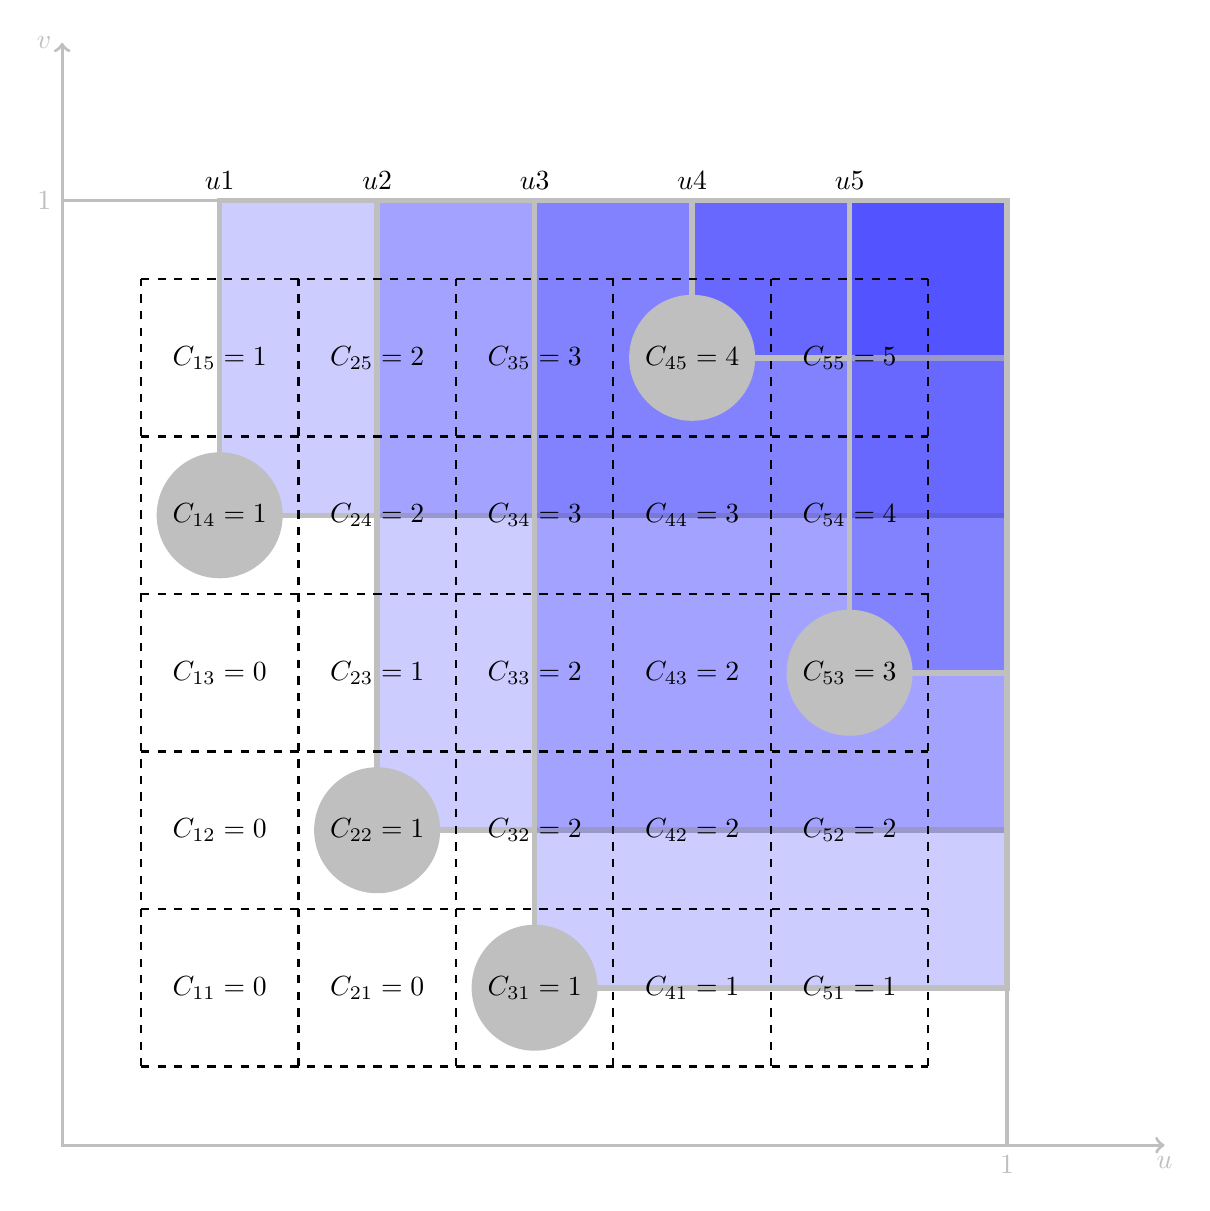
\begin{tikzpicture}[very thick, scale=2]
	\coordinate (A1) at (0,0);
	\coordinate (A2) at (6, 6);
	%\draw [help lines, lightgray] (A1) grid (A2);
	\draw [<->, lightgray] (0, 7) node[left] {$v$} -- (0, 0) -- (7, 0) node[below] {$u$};
	\node[left, lightgray] (u) at (0,6) {1};
	\node[below, lightgray] (v) at (6,0) {1};
	\draw[lightgray] (0,0) rectangle (6,6);


	% points
	\coordinate (unit) at (6,6);
	\foreach \x/\y in {1/4,2/2,3/1,4/5,5/3}{
	\fill[blue, fill opacity=0.2] (\x, \y) rectangle (unit);
	\draw[lightgray, line width=2] (\x, \y) rectangle (unit);
\path[fill=lightgray] (\x,\y) circle (0.4cm);}

	% u axis labels
	\foreach \ind in {1,2,3,4,5}{
	\draw (\ind,6)node[above] {$u$\ind};}

		\node at (1,1) {$C_{11} = 0$};
		\node at (1,2) {$C_{12} =0$};
		\node at (1,3) {$C_{13} = 0$};
		\node at (1,4) {$C_{14} = 1$};
		\node at (1,5) {$C_{15} = 1$};
		\node at (2,1) {$C_{21} = 0$};
		\node at (2,2) {$C_{22} = 1$};
		\node at (2,3) {$C_{23} = 1$};
		\node at (2,4) {$C_{24} = 2$};
		\node at (2,5) {$C_{25} = 2$};
		\node at (3,1) {$C_{31} = 1$};
		\node at (3,2) {$C_{32} = 2$};
		\node at (3,3) {$C_{33} = 2$};
		\node at (3,4) {$C_{34} = 3$};
		\node at (3,5) {$C_{35} = 3$};
		\node at (4,1) {$C_{41} = 1$};
		\node at (4,2) {$C_{42} = 2$};
		\node at (4,3) {$C_{43} = 2$};
		\node at (4,4) {$C_{44} = 3$};
		\node at (4,5) {$C_{45} = 4$};
		\node at (5,1) {$C_{51} = 1$};
		\node at (5,2) {$C_{52} = 2$};
		\node at (5,3) {$C_{53} = 3$};
		\node at (5,4) {$C_{54} = 4$};
		\node at (5,5) {$C_{55} = 5$};

	\draw [thick, dashed, xshift=0.5cm, yshift=0.5cm] (0, 0) grid (5,5);
		
\end{tikzpicture}

\end{document}
